\chapter{Estudo de Caso}

Neste capítulo apresentamos o estudo de caso sobre a utilização de práticas de usabilidade e testes automatizados no desenvolvimento do Portal do Software Público, onde será definido um guia de como essas práticas podem ser inseridas nesse contexto.

O objetivo global desse estudo é introduzir técnicas de usabilidade no desenvolvimento empírico a partir das práticas de BDD.
%
Tendo em vista a utilização de várias técnicas de usabilidade e de testes de software em um projeto de desenvolvimento empírico, definimos os objetivos específicos à fim de:

\begin{enumerate}
\item Avaliar relação entre práticas de BDD e práticas de usabilidade de um software. 

\item Integrar técnicas de usabilidade em um contexto específico de desenvolvimento empírico de software.
\end{enumerate}

Para nos guiarmos  em ralação aos objetivos estabelecidos, definimos as seguintes questões-problemas:

\begin{enumerate}
\item Como os testes automatizados são definidos e implementados em um ambiente de desenvolvimento de software empírico?
\item Como inserir os princípios e técnicas de usabilidade dentro do desenvolvimento empírico de software?
\item Como o processo de desenvolvimento utilizando práticas do BDD podem se relacionar com testes de usabilidade?
\end{enumerate}

Para respondermos as questões-problemas, definimos a seguinte hipótese:

\textbf{Hipótese H1: } A integração de práticas de usabilidade a partir do desenvolvimento por comportamento (BDD) melhor introduz as técnicas de usabilidade no ciclo de desenvolvimento.
	
%ToDo: Explicar a hipotese DONE
Esta hipótese foi definida levando em consideração que o desenvolvimento empírico tem como prática básica os testes automatizados, e em contrapartida se dá pouca atenção à usabilidade. Assim pensamos em utilizar as práticas de testes que já são constantes para introduzir no ciclo as práticas de usabilidade.

\section{Objeto de Estudo}

O Portal do Software Público Brasileiro consiste em um sistema que permite o compartilhamento de softwares e faz parte da política de software livre no setor público.
O SPB será o objeto de estudo de caso, assim como o processo de colaboração com o SPB, que é realizado no LAPPIS da UnB.

O processo de colaboração com o SPB baseia-se no desenvolvimento empírico. O desenvolvimento de testes automatizados é intrínseco ao processo de desenvolvimento, assim buscamos evoluir a forma com que o processo de colaboração com o SPB lida com problemas de usabilidade.
O desenvolvimento é feito a partir de \textit{sprints} de duas semanas, em que são realizadas reuniões com as equipes e reuniões de planejamento (Planning Poker) em cada equipe para definir as atividades de cada \textit{sprint}.

O estudo de caso abrange algumas funcionalidades, que foram desenvolvidas durante o projeto, sendo as seguintes histórias: (1) Cadastro de Usuário, (2) Cadastro de Instituição e (3) Cadastro de Software, que passaram por ciclos de avaliações de usabilidade. 

\subsection{Ciclo 1 de Avaliações}

As avaliações começaram durante a release 2, a partir da sprint 17, seguindo a descrição de avaliação de heurística na seção \ref{metodos_avaliacoes}.
%
Para cada funcionalidade desenvolvida foi determinado um cenário de uso, base para a implementação dos testes de aceitação e consequentemente o seu desenvolvimento.
%
Durante a \textit{release} 1 (sprint 17) foi desenvolvida a história de ``Cadastro de Usuário'', que possui o seguinte cenário de sucesso:

	\begin{itemize}
	\item\textbf{Cenário 01:} Cadastro com sucesso de apenas campos obrigatórios

	\textbf{[Dado]} que não existe nenhum usuário com o nome de usuário ``josesilva''

	\textbf{[Quando]} eu clicar em cadastrar novo usuário

	\textbf{[E]} eu preencho os seguintes campos: 

  		\subitem nome de usuário: ``josesilva''

  		\subitem e-mail: ``jose@gmail.com''

  		\subitem senha: ``123456''

  		\subitem confirmação da senha: ``123456''

  		\subitem nome completo: ``José da Silva''

  		\subitem país: ``Brasil''

  		\subitem estado: ``Distrito Federal''

  		\subitem cidade: ``Brasília''

	\textbf{[E]} eu clico em cadastrar

	\textbf{[Então]} eu recebo uma confirmação de cadastro realizado com sucesso
	\end{itemize}
Outra funcionalidade desenvolvida foi a história chamada ``Manter Instituição'', que possui o seguinte cenário de sucesso:

\begin{itemize}
\item\textbf{Cenário 01:} Cadastro de nova instituição com sucesso

\textbf{[Dado]} que eu estou na página de cadastro de usuário

\textbf{[Quando]} eu clicar em ``Cadastrar nova instituição''

\textbf{[E]} eu preencher os seguintes campos:

  	\subitem sigla: ``MP''

  	\subitem poder: ``executivo''

  	\subitem esfera: ``federal''

  	\subitem tipo: ``pública''

  	\subitem cnpj: ``00.489.828/0002-36''

\textbf{[Então]} eu devo visualizar a mensagem ``Instituição cadastrada com sucesso!''
\end{itemize}
Os demais cenários encontram-se na seção apêndice \ref{cenario_uso}. 

Após desenvolvidos, estes cenários apresentaram alguns problemas de usabilidade na avaliação das heurísticas de Nielsen (seção \ref{metodos_avaliacoes}). Estes problemas estão descritos na tabela \ref{tabela_1a}

%INSERIR TABELA DE PROBLEMAS
\begin{table}[h!]
\label{tabela_1a}
\scalefont{.65}
\begin{tabular}{|l|p{3cm}|p{6cm}|p{3cm}|l|}
\hline
\textbf{ID} & \textbf{Local} & \textbf{Descrição do Problema}                                                                                     & \textbf{Heurística Desobedecida} & \textbf{Criticidade} \\ \hline
1           & Cadastro de Usuário                 & Linguagens estrangeiras e avisos em outros idiomas & Diálogos simples  & Média                \\ \hline
2           & Cadastro de Usuário      & Botão de adicionar nova instituição não é claro para o usuário.  & Minimizar a sobrecarga de memória do usuário;           & Alta                \\ \hline
3           & Cadastro de Usuário               & Diferença entre botão adicionar nova instituição e criar nova instituição para o usuário  & Minimizar a sobrecarga de memória do usuário & Media                \\ \hline
4           & Cadastro de Instituição             & Seleção de País deve ter Brasil como default  & Diálogos simples e naturais    & Baixa                \\ \hline
5           & Cadastro de Instituição      & Opção de escolha do estado: Random button não posicionado e não funciona no primeiro clique. & Diálogos simples e naturais  & Baixa                \\ \hline
6           & Cadastro de Usuário  & Caso você não preencha o email secundário ele informa a seguinte mensagem: E-mail or secondary e-mail already taken & Boas mensagens de erros                & Média                \\ \hline
7           & Cadastro de Usuário  & Opção recaptcha só aparece na segunda vez & Consistência                     & Alta                \\ \hline
8           & Perfil de Usuário  & Ao clicar em hide no bloco de progresso de perfil ele some e não foi encontrada uma opção fácil para reverter a situação.
 & Prevenção de erros                     & Baixa                \\ \hline
9           & Cadastro de Usuário  & Caso se tenha uma infinidade de grupos, fica inviável a opção de checkbox. Ou será utilizada apenas para grupos mais ``conhecidos''? & Atalhos & Média                \\ \hline
10           & Cadastro de Usuário  & Mensagem de erro um pouco confusa: Usuário com este Usuário já existe.  & Consistência                     & Baixa                \\ \hline
\end{tabular}
\caption{Avaliações de usabilidade - sprint 17}
\scalefont{1}
\end{table}

Cada problema levantado nas avaliações gerou uma proposta de melhorias para os cenários envolvidos. Essas melhorias, quando aceitas, geraram mudanças nos cenários de testes de aceitação, consequentemente no desenvolvimento da funcionalidade em si. Os testes de aceitação alterados foram utilizados para verificar os seguintes fatores:

\begin{itemize}
	\item Capacidade de cadastrar informações de usuário;
	\item Capacidade de editar informações de usuário;
	\item Capacidade de cadastrar informações de instituição;
	\item Capacidade de editar informações de instituição;
\end{itemize}

\subsection{Ciclo 2 de Avaliações}

O ciclo 2 de avaliações foi realizado na sprint 18. Durante a \textit{release} 2 a história de ``Cadastro de Usuário'' foi desenvolvida novamente com novo cenário \ref{cenario_r1}. Para este cenário foi desenvolvido o seguinte protótipo, baseando-se nos requisitos definidos pelos clientes. 

	\begin{figure}[h!]
    	\centering
    	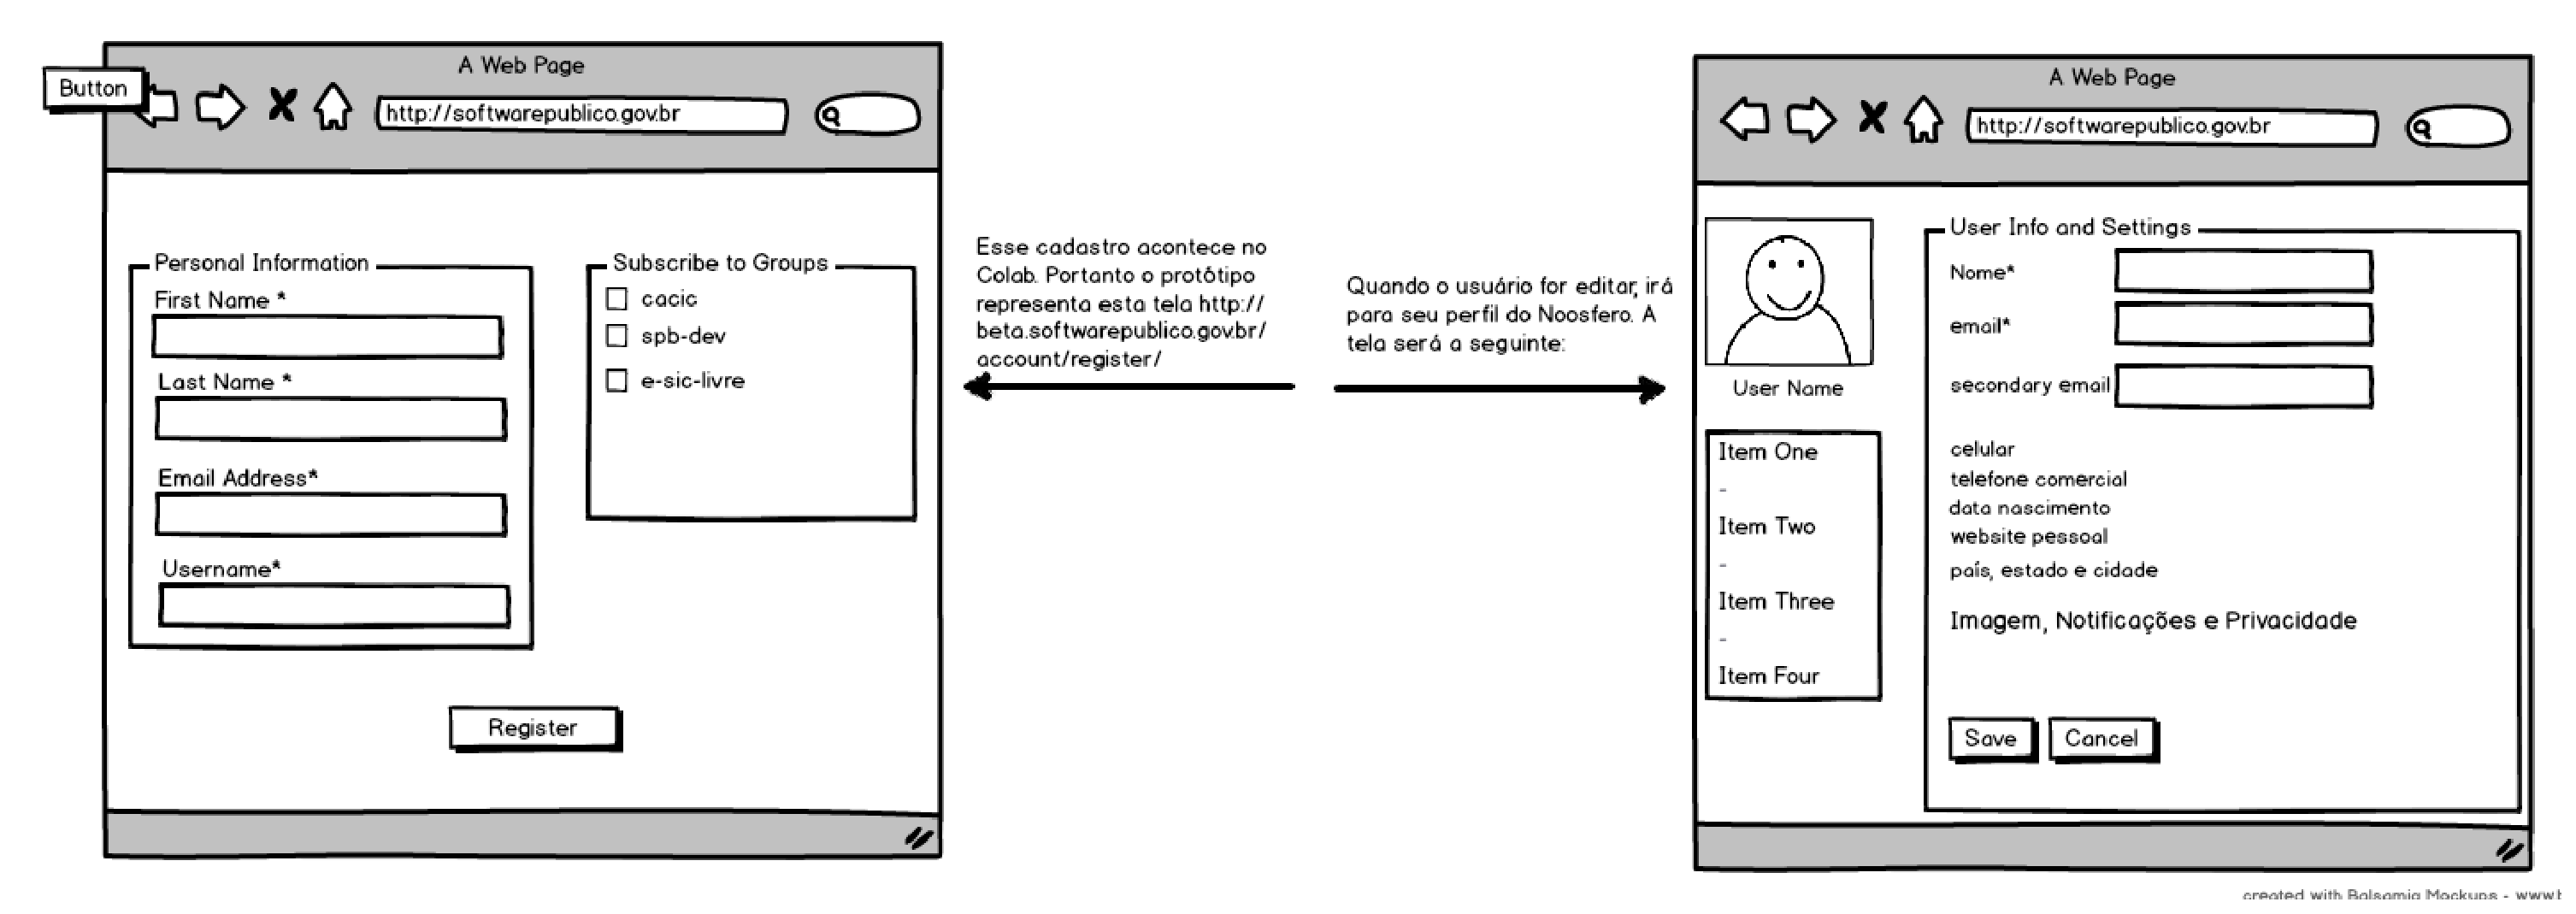
\includegraphics[keepaspectratio=true,scale=0.3]
      		{figuras/CadastroEdicaoUser.eps}
    	\caption{Protótipos de cadastro de usuário}
    	\label{cadastro user}
	\end{figure}

Assim a história de ``Novo Software'' também foi desenvolvida, com o seguinte cenário de sucesso:

\begin{itemize}
\item\textbf{Cenário 01:} Novo Software

	\textbf{[Dado]} que não existe nenhum software com o localhost ``software''

	\textbf{[Quando]} eu clicar em ``Novo Software''

	\textbf{[E]} eu preencho os seguintes campos: 

  		\subitem localhost: ``software''

  		\subitem finalidade: ``Finalidade do software''

  		\subitem licença: ``licença''
  		
  		
	\textbf{[E]} eu clico em ``Salvar''

	\textbf{[Então]} eu recebo uma confirmação de cadastro realizado com sucesso, e encontro a pagina de edição de software
\end{itemize}
Assim como os cenários anteriores, os demais cenários da história de ``Novo Software'' encontra-se em \ref{cenario_r2}. Para esta história também foi desenvolvido um protótipo:

	\begin{figure}[h!]
    	\centering
    	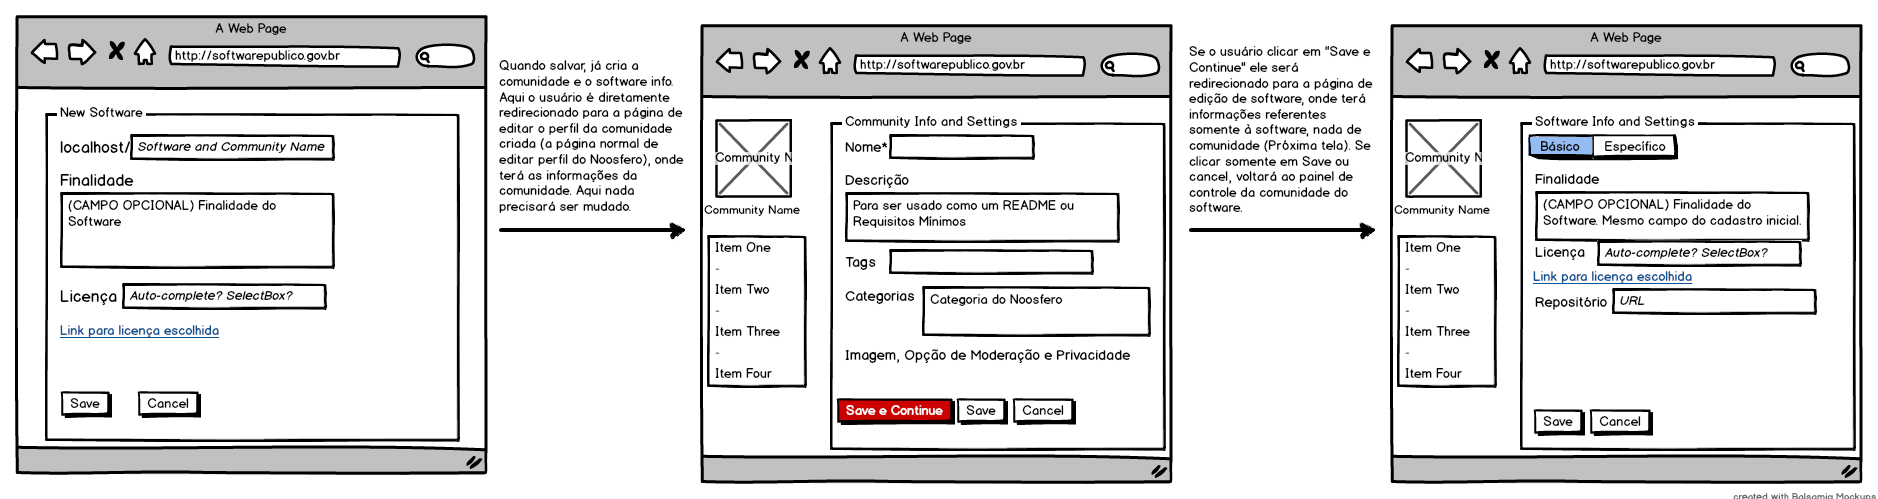
\includegraphics[keepaspectratio=true,scale=0.23]
      		{figuras/CadastroEdicaoSoftware.eps}
    	\caption{Protótipos de cadastro de software}
    	\label{cadastro software}
	\end{figure}


Para dar continuidade ao processo avaliamos os cenários da história de ``Novo Software'' (tabela \ref{table_1a}) durante a sprint 18: 

\begin{table}[h!]
\label{table_1a}
\scalefont{.7}
\begin{tabular}{|l|p{3cm}|p{6cm}|p{3cm}|l|}
\hline
\textbf{ID} & \textbf{Local} & \textbf{Descrição do Problema}                                                                                     & \textbf{Heurística Desobedecida} & \textbf{Criticidade} \\ \hline
1           & Protótipo - Novo Software                 & Ao escolher um nome para o software, não há evidência do que aconteceria caso o nome fosse igual a outro existente & Prevenção de erros               & Média                \\ \hline
2           & Protótipo - Novo Software                 & Não há informação para o usuário do que seria o ``Link''                                                             & Ajuda e documentação             & Média                \\ \hline
3           & Protótipo - Nova Comunidade               & Palavras em inglês e português                                                                                     & Linguagem Clara                   & Baixa                \\ \hline
4           & Protótipo - Nova Comunidade               & Falta de informação sobre as tags e as categorias do noosfero                                                      & Ajuda e documentação             & Baixa                \\ \hline
5           & Protótipo - Novo Software                 & Campos obrigatórios não são definidos                                                                              & Prevenção de erros               & Média                \\ \hline
6           & Protótipo - Novo Software    & Mensagens de ajuda ao preenchimentos dos campos                                                                    & Prevenção de erros               & Baixa                \\ \hline
7           & Protótipo - Nova Comunidade               & Botão de Save e Continue altera estrutura da pagina de software                                                    & Consistência                     & Baixa                \\ \hline
\end{tabular}
\caption{Avaliações de usabilidade - sprint 18}
\scalefont{1}
\end{table}

Cada problema levantado nas avaliações  da sprint 18 gerou uma proposta de melhorias para os cenários envolvidos. Como fizemos as avaliações do segundo ciclo em cima dos protótipos, geramos insumos para o desenvolvimento dos testes de aceitação, que verificam os seguintes fatores:

\begin{itemize}
	\item Capacidade de cadastrar informações software;
	\item Capacidade de editar informações de software;
	\item Capacidade de desativar software;
\end{itemize}

\subsection{Ciclo 3 de Avaliações}

No ciclo 3, realizado durante a sprint 19, aplicamos checklists (\ref{checklist}) para auxiliar nas avaliações e levantamos os seguintes problemas em relação as histórias de ``Cadastro de Usuário'' e ``Cadastro de Software'', na tabela \ref{tabela2a}:

\begin{table}[h!]
\label{tabela2a}
\scalefont{.75}
\begin{tabular}{|l|p{3cm}|p{6cm}|p{3cm}|l|}
\hline
\textbf{ID} & \textbf{Local} & \textbf{Descrição do Problema}                                                                                     & \textbf{Heurística Desobedecida} & \textbf{Criticidade} \\ \hline
1           & Cadastro de Usuário                 & Rótulos dos campos de registro não contém um elemento de convite à entrada de dados ( “ : ”) & Diálogos simples e naturais     & Baixa                \\ \hline
2           & Cadastro de Usuário                 & Usuário não encontra informações suficientes sobre grupos que pode participar  & Diálogos simples e naturais             & Média                \\ \hline
3           & Cadastro de Usuário               & Ao se excluir um e-mail secundário, não existe solicitação de confirmação       & Feedback                & Alta                \\ \hline
4           & Cadastro de Software     & Dificuldade para acessar o botão de criar software
	        & Minimizar sobrecarga          & Baixa                \\ \hline
5           & Cadastro de Software       & Funcionalidade de criar software também cria comunidade, porém o usuário não é informado disto  & Feedback    & Média                \\ \hline
6           & Cadastro de Software    & Dificuldade para acessar o botão de editar software
		    & Minimizar sobrecarga           & Baixa                \\ \hline
7           & Cadastro de Software    & Fluxo de edição não está claro (etapas)
			& Feedback                       & Média                \\ \hline
8           & Cadastro de Software    & frase ``The highlighted fields are mandatory'' não especifica o char (*)
		    &Diálogos simples e naturais     & Baixa                \\ \hline
\end{tabular}
\caption{Avaliações de usabilidade - sprint 19}
\scalefont{1}
\end{table}

Após as melhorias propostas serem desenvolvidas e longo do processo de evolução das histórias mencionadas, os testes de aceitação foram utilizados para verificar os seguintes fatores:

\begin{itemize}
	\item Capacidade editar informações de usuário;
	\item Capacidade de registrar informações de software;
	\item Capacidade de desativar usuário;
	\item Capacidade de validar software público;
\end{itemize}


\section{Análise e Interpretação dos Resultados}
\label{analise}

Analisamos a evolução de cada história ao longo dos ciclos de avaliações. Cada ciclo de avaliação representa um sprint, em que foram realizadas as avaliações. O ciclo 1 foi realizado na sprint 17, o ciclo 2 na sprint 18 e o ciclo 3 na sprint 19. Uma das histórias avaliadas foi a de ``Cadastro de Usuário'':


\begin{figure}[h!]
    	\centering
    	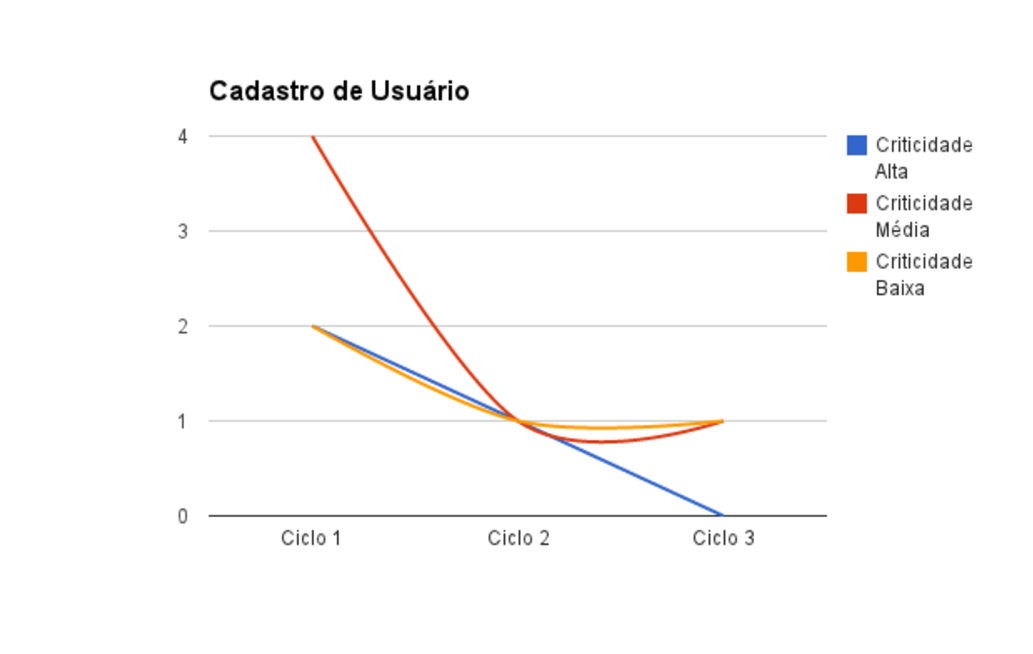
\includegraphics[keepaspectratio=true,scale=0.62]
      		{figuras/graf01.eps}
    	\caption{Resultado das avaliações de ``Cadastro de Usuário''}
    	\label{avaliacaouser}
\end{figure}

Já em ``Cadastro de Instituição'', temos:

\begin{figure}[h!]
    	\centering
    	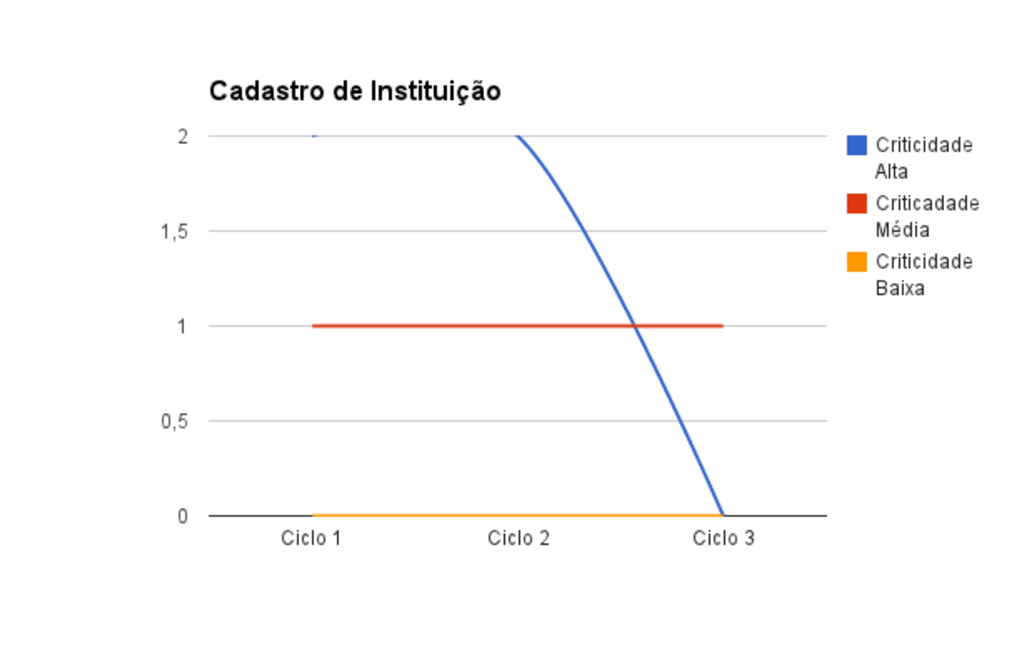
\includegraphics[keepaspectratio=true,scale=0.62]
      		{figuras/graf02.eps}
    	\caption{Resultado das avaliações de ``Cadastro de Instituição''}
    	\label{avaliacaoinstitucion}
\end{figure}

Quanto à história de ``Cadastro de  Software'', temos:

\begin{figure}[h!]
    	\centering
    	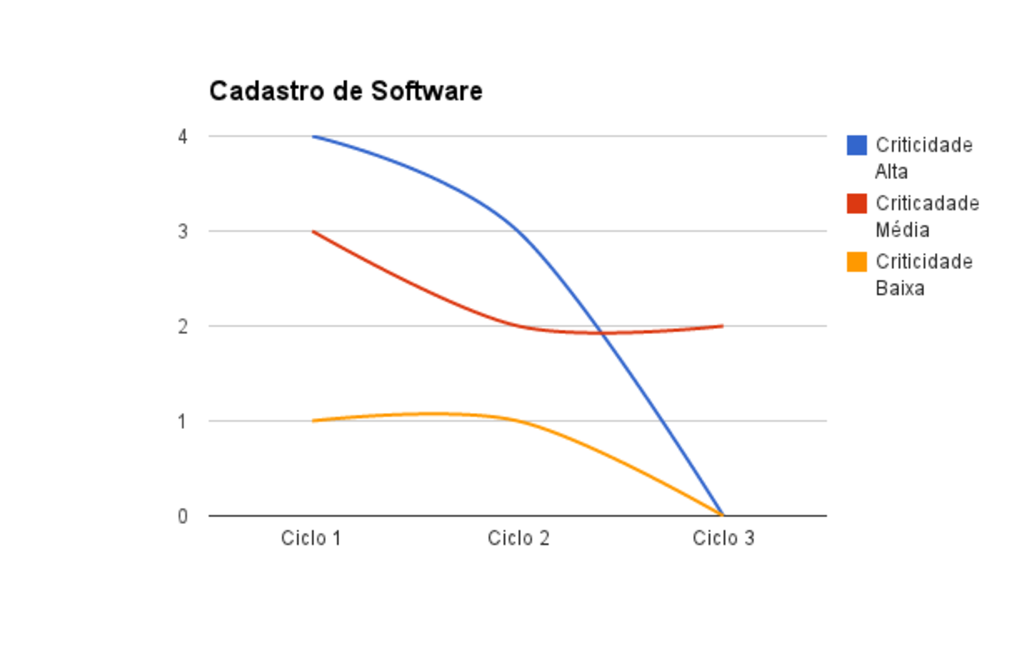
\includegraphics[keepaspectratio=true,scale=0.62]
      		{figuras/graf03.eps}
    	\caption{Resultado das avaliações de ``Cadastro de Software''}
    	\label{avaliacaosoftware}
\end{figure}

\newpage
Quanto aos testes de aceitação dos cenários avaliados tivemos os seguintes resultados de medição:
%Falta a historia cadastro de instituiçao
História: ``Cadastro de Usuário'':
\begin{itemize}
	\item Quantidade de cenários executados: 22 cenários;
	\item Quantidade de passos executadas: 162 passos
	\item Quantidade de falhas obtidas: 0 falhas;
\end{itemize} 

História: ``Cadastro de Instituição'':
\begin{itemize}
	\item Quantidade de cenários executados: 2 cenários;
	\item Quantidade de passos executadas: 23 passos
	\item Quantidade de falhas obtidas: 0 falhas;
\end{itemize} 

História: ``Cadastro de Software'':
\begin{itemize}
	\item Quantidade de cenários executados: 6 cenários;
	\item Quantidade de passos executadas: 68 passos
	\item Quantidade de falhas obtidas: 0 falhas;
\end{itemize} 

\section{Inserção das Práticas de Usabilidade}

Durante o estudo de caso inserimos algumas práticas ( prototipação, checklist e avaliação de heurísticas) de usabilidade no objeto de estudo, integrando com práticas de métodos empíricos já utilizadas como os testes de aceitação. A prototipação é feita durante o lenvantamento de requisitos com base nos cenários de testes, esses protótipos devem ser submetidos aos checklists \ref{checklist}, que serão usados como base para as avaliações de heurísticas. As avaliações devem apresentar os problemas de usabilidade, que devem ser utilizadas como insumo para possíveis atividades de melhorias e verificar a implementação das melhorias através dos testes de aceitação, tornando possível o início de um novo ciclo:

\begin{enumerate}
	\item \textbf{Elaboração dos cenários de uso/testes} levantados a partir dos requisitos do sistema;
	\item \textbf{Criação dos protótipos} de acordo com cenários;
	\item \textbf{Aplicação dos checklists} \ref{checklist} nos protótipos criados;
	\item \textbf{Avaliação de heurística} nos protótipos criados, com o auxílio dos resultados dos checklists, levantando problemas de usabilidade;
	\item \textbf{Propor atividades de melhorias} para cada problema levantado durante as avaliações;
	\item \textbf{Verificação pelos testes de aceitação } de cada atividade de melhoria implementada;
	\item \textbf{Reinício do ciclo no item 1;} 
\end{enumerate}

Estes passos estão ilustrados na figura \ref{diagrama1}.

\begin{figure}[h!]
    	\centering
    	\includegraphics[keepaspectratio=true,scale=0.35]
      		{figuras/diagrama.eps}
    	\caption{Atividades do estudo de caso}
    	\label{diagrama1}
\end{figure}

Com este ciclo possibilitamos a inserção de práticas de usabilidade de forma empírica, diminuindo assim a curva de apredizagem da equipe e agregando a importância da usabilidade no processo de desenvolvimento.

\section{Considerações}

Este capítulo apresentou o estudo de caso sobre o desenvolvimento do Portal do Software Público a partir de métodos empíricos, utilizando práticas de BDD e usabilidade.

